%%%%%%%%%%%%%%%%%%%%%%%
% PACKAGES NECESSÁRIOS
%%%%%%%%%%%%%%%%%%%%%%%
\documentclass[12pt,brazil,a4paper]{article}
\usepackage[portuguese]{babel}
\usepackage[utf8]{inputenc}
\usepackage{tcolorbox}
\usepackage[export]{adjustbox}
\usepackage{wrapfig}


%%%%%%%%%
% ARTIGO
%%%%%%%%%
\begin{document}
\title{\textbf{Covid for Kids}}
\author{Alexya Oliveira, Gabriel Fanto Stundner, Lucas Leal, Matheus Santos \\ \\ Pontifícia universidade Católica do Rio Grande do Sul \\ Escola Politécnica \\ Curso de Engenharia de Software}
\maketitle

\textbf{Design de Interação 2020/1}

\textit{Prof. Sílvia Moraes}


\section{Sumário}
\begin{description}
Gerar Indice Aqui
\end{description}
\section{Contexto e Objetivo}
\begin{description}
Propostas de Interface
\end{description}
\section{Escopo e Requisitos}
\begin{description}
Elabore uma breve descrição do projeto e seu escopo. Descreva a abordagem que será usada (gamificação, quiz, atividades, ...). Se o projeto ainda não tiver nome, batize-o. 
\end{description}
\subsection{Requisitos Funcionais}
\begin{tcolorbox}
\textbf{Nome: } Exibir de forma lúdica e pedagógica informações úteis sobre o vírus e prevenção \\
\textbf{Descrição: } \\
\tab\tab \textbf{Como: } Criança    \\
\tab\tab \textbf{Eu quero: } Jogar um jogo de luta contra o Corona vírus\\
\tab\tab \textbf{Para que: } Eu possa aprender formas de prevenção na quarentena\\
\textbf{Notas: } \\
\textit{a) } O jogo tem que ser simples para crianças\\
\textit{b) } O jogo tem que ser didático   
\end{tcolorbox}
\subsection{Requisitos Não-Funcionais}
\section{Modelos de Usuário}
\begin{description}
Quem são os usuários (atuais e futuros) ?” 
\end{description}
\subsection{Perfil de Usuários}
\subsection{Personas}
\subsubsection{Pedro Henrique}
\textbf{Pedro Henrique, 10 anos, Ensino Fundamental}\\
\textit{Stakeholder Primário}\\
Pedro Henrique é um Estudante do Ensino Fundamental que se encontra em quarentena devido á um Pandemia do COVID-19 e por 
isso não pode ir para as aulas, tendo que ficar em casa sem entender o motivo de tudo isso, como a mãe dele não deixa
ele assistir televisão devido as más noticias ele gostaria de entender o que está acontecendo e poder conversar com os amigos dele.\\
\begin{wrapfigure}{l}{0.25\textwidth}
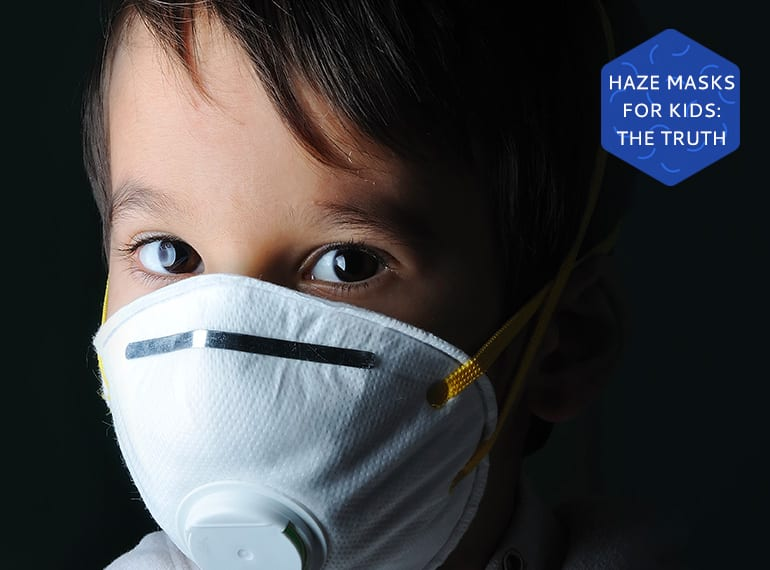
\includegraphics[width=1.0\linewidth]{children_1.jpg}
\end{wrapfigure}
Pedro Henrique gosta muito de Jogos, que o fazem companhia nesse momento que tem de ficar em casa, então ficou interessado em saber
se existe algum Jogo em casa que ele pode aprender mais sobre essa Quarentena e poder se divertir e aprender algo enquanto
espera voltar para as aulas.\\
\subsubsection{Pâmela Medeiros}
\textbf{Pâmela Medeiros, 11 anos, Estudante de Casa}\\
\textit{Stakeholder Primária}\\
Pãmela Medeiros é uma Estudante de Casa desde pequena. Os pais delas são cientistas que estão tentando
descobrir uma cura para o Vírus COVID-19 e acabar com a Pândemia.
Como Pâmela é uma Aluna Brilhante, ela entende que existem muitas crianças que não entendem o que está acontecendo no mundo
e estão em casa com medo por causa dos Adultos que não explicam o que está acontecendo.
\begin{wrapfigure}{l}{0.25\textwidth}
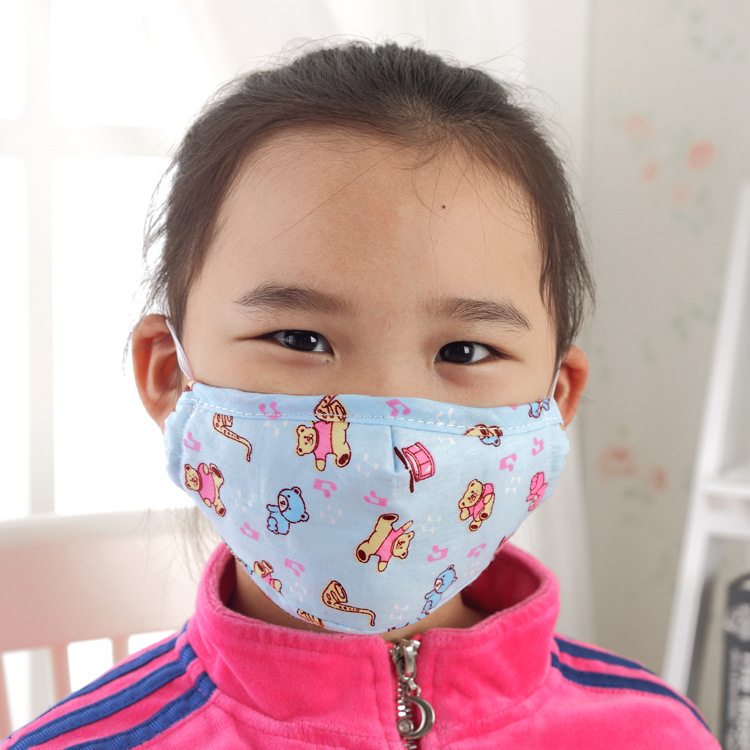
\includegraphics[width=0.9\linewidth]{children_2.jpg}
\end{wrapfigure}
Assim como muitas crianças da idade da Pâmela, ela adora Jogar e sabe que Jogos para os jovens é a melhor forma de ensinar
quando as outras formas não conseguem. Com essa idéia na cabeça ela começou a estudar formas de ensinar as outras crianças
a se cuidarem em casa para não ficarem doentes, ensinando através de joguinhos que ela conhece ou criou, mas ela só
consegue ensinar as crianças na volta dela, para isso ela precisa de algum aplicativo de celular ou de internet onde
ela possa apresentar para as outras crianças do mundo todo para se cuidarem nesse momento tão dificil.
\subsubsection{Martha Silva}
\textbf{Martha Silva, 24 anos, Estudante de Medicina}\\
\textit{Stakeholder Secundário}\\
Martha Silva é uma Estudante de Medicina na Faculdade PUCRS em Porto Alegre,Rio Grande do Sul, Brasil.
Martha teve um filho muito cedo, que hoje tem 6 anos de idade, e se preocupa muito com ele todos os dias enquanto trabalha
no Hospital salvando vidas. Como é um assunto muito delicado ela não sabe explicar muito bem pro filho dela o porque
a Mãe dele está morando longe de casa por muitos dias e ela sabe que não existe uma forma fácil de mostrar o porque
que o mundo está em uma Pandemia. 
\begin{wrapfigure}{l}{0.25\textwidth}
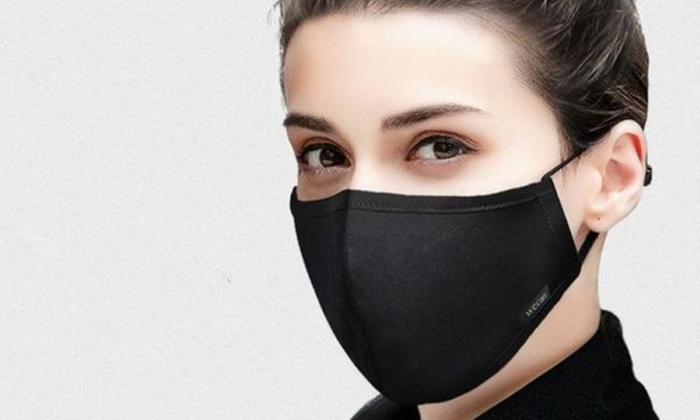
\includegraphics[width=1.0\linewidth]{adult_1.jpg}
\end{wrapfigure}
Dessa forma ela precisava encontrar algum Jogo ou desenho que explica-se a ausência dela
por tantos dias e ao mesmo tempo ensinar o filho dela o porque é importante se cuidar da Higiene todo 
o tempo para que não fica-se doente, dessa forma não só o filho dela estaria bem informado nas formas de Higiene
como também iria se divertir um pouco já que se encontra em casa o dia todo devido ao fechamento das escolas.
\section{Modelos de Trabalho}
\begin{description}
\subsection{Personas}

\end{description}
\section{Prototipação}
\begin{description}
Organizar em subseções para descrever os itens do enunciado.
\end{description}
\section{Avaliação}
\begin{description}
Descrição da avaliação do protótipo. Realizar a avaliação junto aos usuários e documentar o feedback. Indicar ainda as melhorias feitas no protótipo que foram decorrentes da avaliação dos usuários e do stakeholder.
\end{description}
\section{Considerações Finais}
\begin{description}
Comentar o trabalho, no que ele contribuiu para sua aprendizagem e as dificuldades encontradas.
\end{description}




\end{document}